% !TeX root = ../Book1.tex
\begin{figure}[htbp]
	\centering
	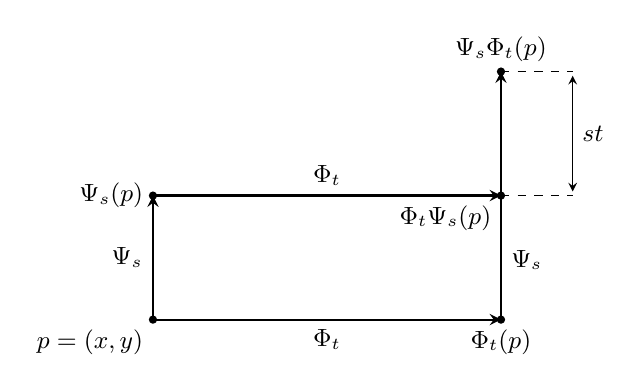
\begin{tikzpicture}[>=stealth,x=1.3cm,y=1.05cm,font=\small]
		\coordinate (P) at (0,0);
		\coordinate (XP) at (3.4,0);
		\coordinate (YP) at (0,1.5);
		\coordinate (XYP) at (3.4,1.5);
		\coordinate (YXP) at (3.4,3);
		\draw[->,thick] (P)--node[below] {\(\Phi_t\)} (XP);
		\draw[->,thick] (P)--node[left] {\(\Psi_s\)} (YP);
		\draw[->,thick] (YP)--node[above] {\(\Phi_t\)} (XYP);
		\draw[->,thick] (XP)--node[right,pos=.24] {\(\Psi_s\)} (YXP);
		\draw[dashed] (XYP)--(4.1,1.5);
		\draw[dashed] (YXP)--(4.1,3);
		\draw[<->] (4.1,1.55)--node[right] {\(st\)} (4.1,2.95);
		\foreach \Q in {P,XP,YP,XYP,YXP} \fill (\Q) circle (1.5pt);
		\node[below left] at (P) {\(p=(x,y)\)};
		\node[below] at (XP) {\(\Phi_t(p)\)};
		\node[left] at (YP) {\(\Psi_s(p)\)};
		\node[below left] at (XYP) {\(\Phi_t\Psi_s(p)\)};
		\node[above] at (YXP) {\(\Psi_s\Phi_t(p)\)};
	\end{tikzpicture}
	\caption{\(X=\partial_x\)、\(Y=x\partial_y\) 的两种运动次序，图中以 \(x,s,t>0\) 示意。先作水平运动会增加随后竖直运动的速度，两个终点的竖直差为 \(st\)。}
	\label{g1:fig:flow-order}
\end{figure}
